\documentclass{beamer}
%\documentclass[handout]{beamer}

\usepackage{ensislides}
\usepackage[utf8]{inputenc}
\usepackage[french]{babel}


\title[Version courte du titre]{Gestion d'un parc d'imprimantes}

\subtitle{Un exemple} % (optional)

\author{       
                     AGUILAR ARREOLA Laura Elizabeth\\
                     CHAABOUNI Kais\\
                     LEON RODRIGUEZ Eduardo Alberto\\
                     NAZ André\\}
% - Use the \inst{?} command only if the authors have different
%   affiliation.

\institute{Ensimag}

\date{2012-2013}

\begin{document}

\begin{frame}
  \titlepage
\end{frame}

\section{Conception}

\subsection{Dépendance fonctionnelles}

\begin{frame} \frametitle{Dépendances fonctionnelles}

        %\begin{table}[h]
          %\fontfamily{cmtt}\selectfont
         % \setlength{\tabcolsep}{1pt}
\tiny
          \begin{tabular}{p{10cm}}
            \{idCopieur$\} \rightarrow$  \{nom, marque, modele, emplacement,
            niveauEncreNoire, coutParPage, niveauEncreMagenta,niveauEncreCyan, niveauEncreJaune\}\\
            \\
            \{idCompte$\} \rightarrow$  \{nomCompte, dureeValidite, CI, CImensuel\}\\
            \\
            \{idCompteGroupe$\} \rightarrow$  \{nomGroupe, idResponsable, participantes\}\\
            \\
	    \{idCompteIndividuel$\} \rightarrow$  \{login, mdp, typeUtilisateur\}\\
	    \\
            \{login $\} \rightarrow$  \{mdp, idCompteIndividuel\}\\
            \\
            \{idDescription, idCompte$\} \rightarrow$  
            \{dateSoumission, nomFichier, format, nbPages, optionsImpression, taillePS, idPS\}\\
            \\
            \{idPS$\} \rightarrow$  \{contenuPS\}\\
            \\
            \{idCopieur, idCompte, idDescription$\} \rightarrow$  \{dateImpression, qteEncreNoire\}\\
            \\
            \{idCopieurCouleur, idCompte, idDescriptionCouleur$\} \rightarrow$  \{
            qteEncreMagenta, qteEncreCyan, qteEncreJaune\}\\
          \end{tabular}
        %\end{table}
        \pause
  \begin{itemize}
  \item {\tt FN1: tout attribut doit avoir une valeur atomique}
        \pause
  \item {\tt FN2: Pas de dépendance partielle}
        \pause
  \item {\tt FN3: Pas de transitivité}
        \pause
  \item {\tt FN3BCK: Partie gauche des DF sont des clés primaires}
  \end{itemize}
\end{frame}

%\begin{frame} \frametitle{Diagramme Entité/Association}
%  \begin{itemize}
%  \item {\tt pdflatex example.tex}
%    \pause
%  \item {\tt pdflatex example.tex} (pour la table des matières)
%  \end{itemize}
%  \pause
%  \question{Ça vous plait ?}
%\end{frame}

\subsection{Diagramme Entité/Association}

\begin{frame} %\frametitle{Diagramme Entité/Association}
        \begin{figure}[h!]
          \begin{center}
            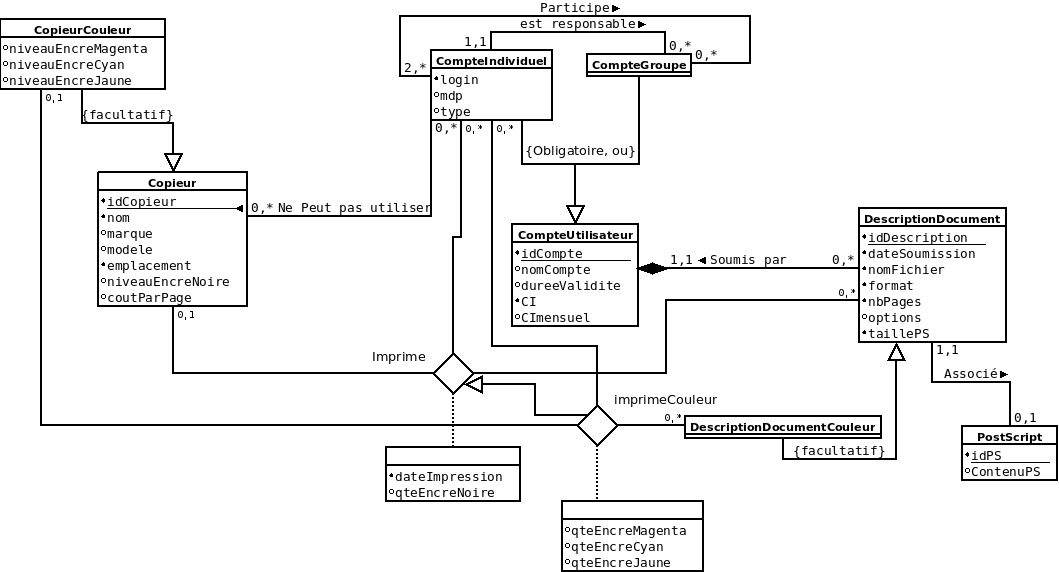
\includegraphics[width=1\textwidth]{diagramme.png}
            \caption{Diagramme Entité/Association}
          \end{center}
        \end{figure}

\end{frame}


\subsection{Modèle logique}

\begin{frame}
  \frametitle{Modèle logique}
\tiny
 \begin{tabular}{p{\textwidth}}
            Copieur(\underline{idCopieur}, nom, marque, modele, emplacement, niveauEncreNoire, coutParPage)\\
            \\
            CopieurCouleur(\underline{idCopieur}$^{\#}$, niveauEncreCyan, niveauEncreMagenta, niveauEncreJaune)\\
            \\
            CompteUtilisateur(\underline{idCompte}, nomCompte, dureeValidite, CI, CImensuel)\\
            \\
            CompteIndividuel(\underline{idCompte}$^{\#}$, login, mdp, typeUtilisateur)\\
            \\
            CompteGroupe(\underline{idCompteGroupe}$^{\#}$, idResponsable$^{\#}$)\\
            \\
            Participe(\underline{idCompteGroupe}$^{\#}$, \underline{idCompteIndividuel}$^{\#}$)\\
            \\
            NePeutPasUtiliser(\underline{idCompte}$^{\#}$, \underline{idCopieur}$^{\#}$)\\
            \\
            DescriptionDocument(\underline{idDescription}, \underline{idCompte}$^{\#}$, dateSoumission, nomFichier, 
            format, nbPages, options, taillePS)\\
            \\
            PostScript(\underline{idPS}, idDescription$^{\#}$, idCompte$^{\#}$, contenu)\\
            \\
            DescriptionDocumentCouleur(\underline{idDescription}$^{\#}$, \underline{idCompte}$^{\#}$)\\
            \\
            Imprime(\underline{idCompte}$^{\#}$, \underline{idDescription}$^{\#}$,\underline{idCompteDescription}$^{\#}$, 
            idCopieur$^{\#}$, dateImpression, qteEncreNoire)\\
            \\
            ImprimeCouleur(\underline{idCompte}$^{\#}$, \underline{idDescription}$^{\#}$, \underline{idCompteDescription}$^{\#}$, 
             qteEncreCyan, qteEncreMagenta, qteEncreJaune)\\
            \\
            
          \end{tabular}

\end{frame}

\section[Deux]{Implantation}

\begin{frame}
  \frametitle{Implantation des fonctionnalités}
 \begin{itemize}
\item Respect de la cohérence
\item Delete on cascade sur les références
\item Transactions de vérification des contraintes
\item Niveau d'isolation: Read commited
\end{itemize}
\end{frame}

\begin{frame}
  \frametitle{Impression}
\end{frame}

\begin{frame}
  \frametitle{Encore un ...}
\end{frame}

\begin{frame}
  \frametitle{Administration}
\begin{itemize}
\item Requètes simples pour localisation encres faibles
\item Droit d'accès: \verb+NEPEUTPASUTILISER+
\item Gestion des utilisateurs
  \begin {itemize} 
\item Compte Individuel
\item Compte Groupe (Responsable, membres, )
  \end {itemize}
\end{itemize}
\end{frame}

\begin{frame}
  \frametitle{Encore un ...}
\end{frame}


\section[Trois]{Démonstration}

\begin{frame}
  \frametitle{Et un dernier}
\end{frame}

\end{document}


%%% Local Variables: 
%%% mode: latex
%%% TeX-master: t
%%% End: 
